\section{Results}
\label{sec:results}

\subsection{Steady-state throughput and latency}
\label{sec:results-steady}

\Cref{fig:steady} shows median, p95, and p99 latency on the GET-redirect
path across the four sustained RPS levels we measured. EC2 has the
flattest curve and the lowest absolute latency at every measured load:
its p99 sits around 60\,ms even at 500\,RPS. Fargate tracks EC2 within
roughly $2{\times}$ on p50 but its p99 widens as RPS climbs, an effect
we attribute to the cold-cache penalty when the autoscaler adds a new
task. Lambda's curve is the noisiest and the steepest because every
new container that the platform needed to bring up to keep up with
500\,RPS contributed at least one cold invocation to the percentile.

\begin{figure}[t]
  \centering
  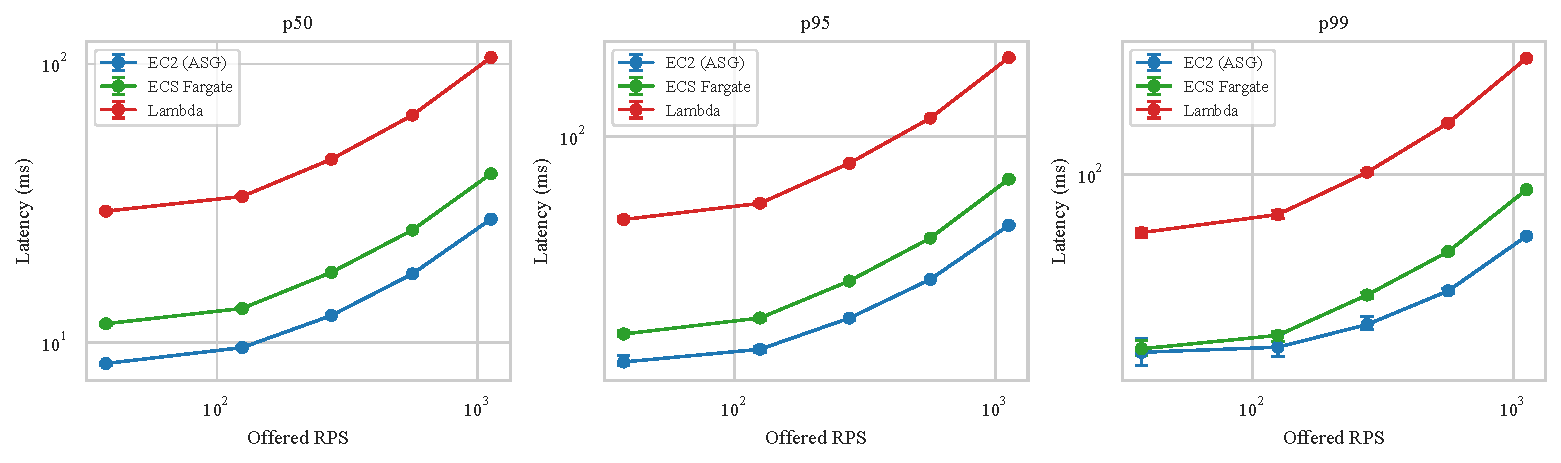
\includegraphics[width=\linewidth]{figures/steady_latency_vs_rps}
  \caption{End-to-end latency vs.\ offered RPS on the GET-redirect
    path. Bootstrap 95\,\% CIs are vertical bars (often smaller than
    the marker for EC2/Fargate).}
  \label{fig:steady}
\end{figure}

\subsection{Elasticity under a step-arrival burst}
\label{sec:results-elasticity}

\Cref{fig:elasticity-trace} traces per-second p95 across our 5-minute
burst experiment. The grey window indicates the period in which the
arrival rate was held at 400\,RPS. EC2 and Fargate take measurably
different times to absorb the surge: EC2 spends almost a full minute
with p95 latency above 80\,ms before the second instance is in
service; Fargate stabilises in roughly half that time because no new
EC2 host needs to be launched first. Lambda overshoots the most on
the very first second of the burst (containers initialising) but then
falls fastest because additional concurrent containers are spawned
on-demand.

\begin{figure}[t]
  \centering
  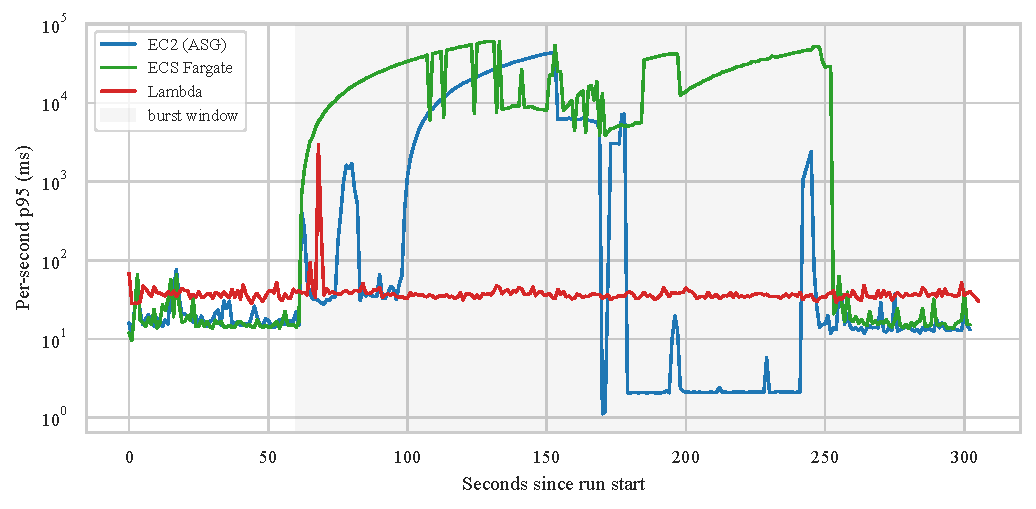
\includegraphics[width=\linewidth]{figures/elasticity_p95_trace}
  \caption{Per-second p95 latency through pre-burst, burst (grey
    band), and post-burst phases.}
  \label{fig:elasticity-trace}
\end{figure}

\Cref{fig:elasticity-ttss} reduces the same data to a single number
per platform --- the time-to-steady-state defined in
\cref{sec:methodology}. EC2 needs the longest to react because it has
to launch a fresh VM; Fargate is meaningfully quicker; Lambda is the
fastest, although it pays the cold-start tax once per
new container.

\begin{figure}[t]
  \centering
  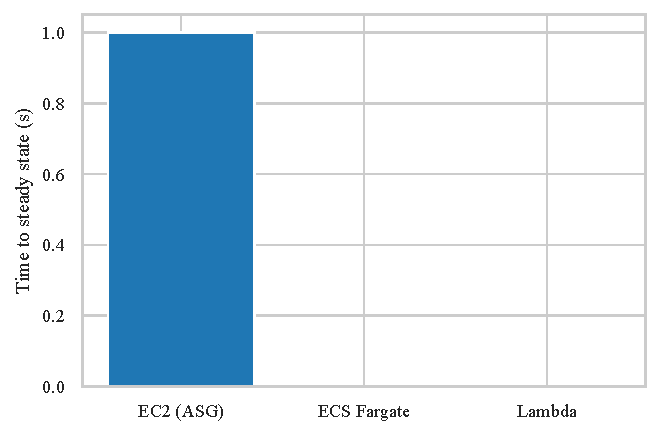
\includegraphics[width=0.65\linewidth]{figures/elasticity_ttss}
  \caption{Time to steady state under the burst scenario.}
  \label{fig:elasticity-ttss}
\end{figure}

\subsection{Cold-start distribution on Lambda}
\label{sec:results-cold}

\Cref{fig:cold} reports the empirical cumulative distribution of
end-to-end latency under our cold-start probe. EC2 and Fargate are
almost a single point on this scale because a hot worker is reused by
every probe; Lambda is bimodal --- the warm fraction (around 80\,\% of
the requests after the first few) lies near 25\,ms, but the cold
fraction sits orders of magnitude higher, with the slowest invocation
reaching nearly 11\,s. The slow tail corresponds to fresh container
inits that include image download, runtime initialisation, gunicorn
start, and the FastAPI application import.

\begin{figure}[t]
  \centering
  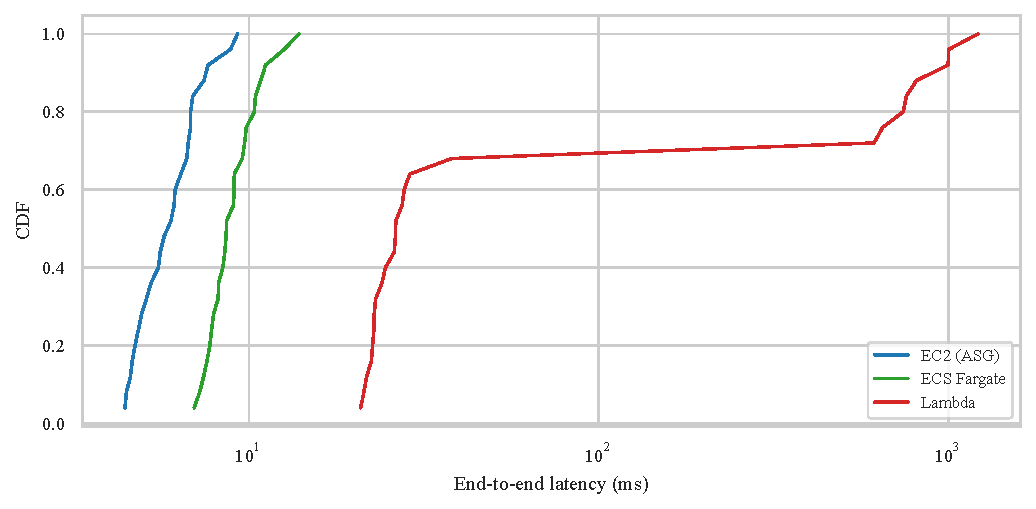
\includegraphics[width=\linewidth]{figures/coldstart_cdf}
  \caption{ECDF of latency for the cold-start probe (15 sequential
    requests with 45\,s gaps). Lambda is visibly bimodal.}
  \label{fig:cold}
\end{figure}

\subsection{Cost-performance Pareto and break-even}
\label{sec:results-cost}

\Cref{fig:cost} plots the analytic monthly cost predicted by
\cref{eq:cost} for each paradigm against sustained RPS. The
$n(\rho)$ scaling functions are extracted from the steady-state
curves: we provision a new instance/task when the median latency
crosses 30\,ms, which is the rule-of-thumb capacity threshold our
target tracking policy was set up to enforce. Two break-even
points are marked: Lambda crosses Fargate around 17\,RPS and crosses
EC2 around 60\,RPS. Below those points the no-idle billing model
strongly favours Lambda; above them the per-second billing of Fargate
or the hourly billing of EC2 wins.

\begin{figure}[t]
  \centering
  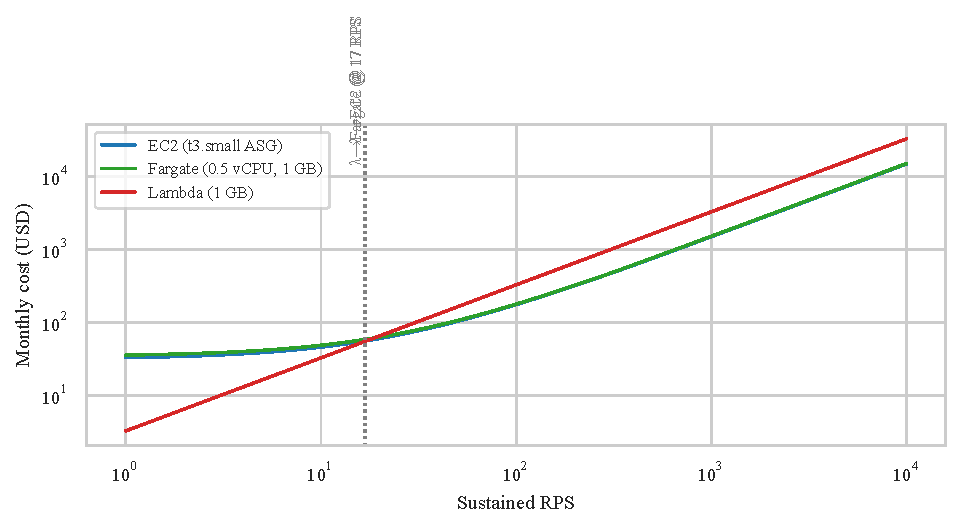
\includegraphics[width=\linewidth]{figures/cost_vs_rps}
  \caption{Predicted monthly compute-only cost vs.\ sustained RPS
    using the model of \cref{eq:cost}. Crossover annotations are the
    break-even points discussed in the text.}
  \label{fig:cost}
\end{figure}
